\documentclass[10pt]{article}
\usepackage[utf8]{inputenc}
\usepackage{xcolor}
\usepackage{helvet}
\renewcommand{\familydefault}{\sfdefault}
\usepackage{tikz}
\usepackage[paperwidth=37cm,paperheight=34cm,left=1cm,right=1cm,bottom=1cm,top=1cm]{geometry}
\usetikzlibrary{mindmap,backgrounds}

\pagestyle{empty}
\begin{document}
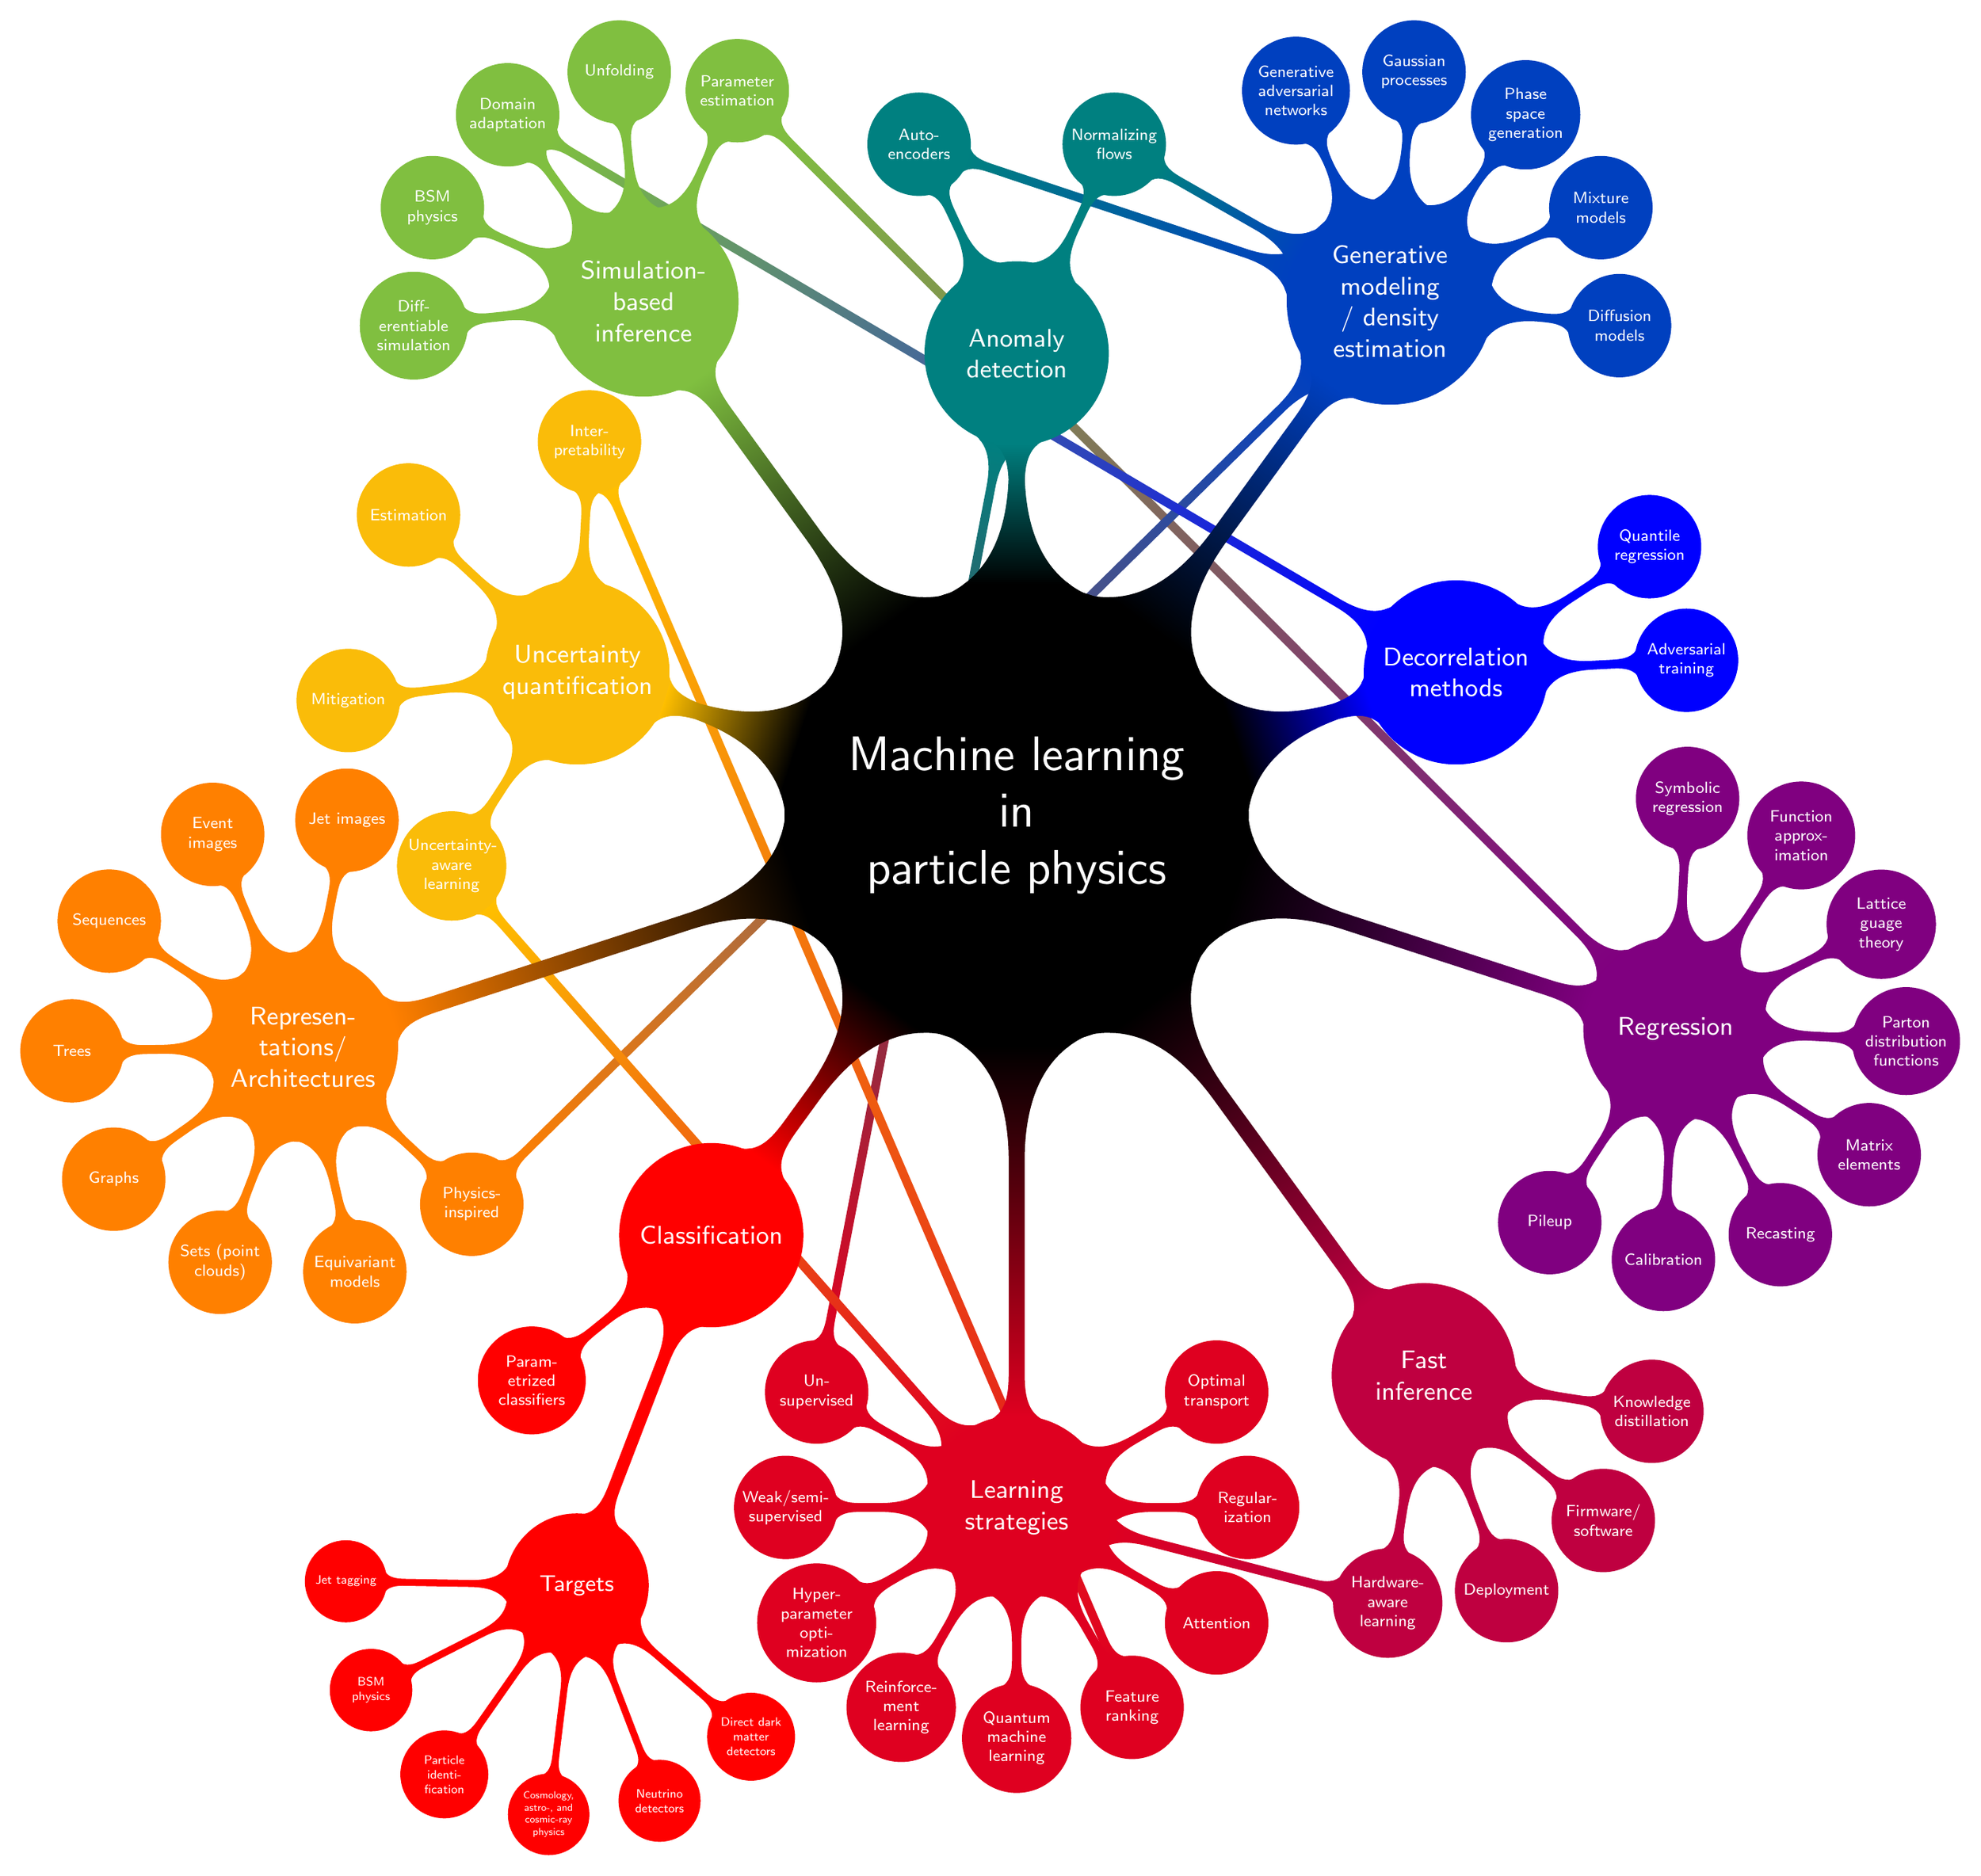
\begin{tikzpicture}[mindmap, grow cyclic, every node/.style=concept, concept color=black, text=white, scale=1,
		level 1/.append style={level distance=8cm,sibling angle=36},
		level 2/.append style={level distance=4cm,sibling angle=30},
		level 3/.append style={level distance=4cm,sibling angle=28},
	]

	\node [scale=2] {Machine learning\\in\\particle physics}
	child [concept color=orange, style={level distance=13cm}] {node  [scale=1.4] {Represen-tations/\\Architectures}
			child [sibling angle=34] {node {Jet images}}
			child [sibling angle=34] {node {Event images}}
			child [sibling angle=34] {node {Sequences}}
			child [sibling angle=34] {node {Trees}}
			child [sibling angle=34] {node {Graphs}}
			child [sibling angle=34] {node {Sets (point clouds)}}
			child [sibling angle=34] {node {Equivariant models}}
			child [sibling angle=34] {node (pinn) {Physics-inspired}}
		}
	child [concept color=red, level distance=9cm] { node [scale=1.4] {Classification}
			child {node  {Param-etrized classifiers} }
			child [style={level distance=6.5cm}]{node [scale=1.4] {Targets}
					child {node [scale=1.2] {Jet tagging}}
					child {node [scale=1.2] {BSM physics}}
					child {node [scale=1.2] {Particle identification}} child {node {Cosmology, astro-, and cosmic-ray physics}}
					child {node [scale=1.2] {Neutrino detectors}}
					child {node [scale=1.2] {Direct dark matter detectors}}
				}
		}
	child [concept color=red!50!purple, style={level distance=12cm}] {node  [scale=1.4] (ls) {Learning strategies}
			child {node (un) {Un-supervised}}
			child {node {Weak/semi-supervised}}
			child {node {Hyper-parameter optimization}}
			child {node {Reinforce-ment learning}}
			child {node {Quantum machine learning}}
			child {node (fr) {Feature ranking}}
			child {node {Attention}}
			child {node {Regular-ization}}
			child {node {Optimal transport}}
		}
	child [concept color=red!50!violet, style={level distance=12cm}] { node [scale=1.4] {Fast\\inference}
			child { node (hal) {Hardware-aware learning}}
			child { node  {Deployment}}
			child { node  {Firmware/\\software}}
			child { node  {Knowledge distillation}}
		}
	child [concept color=violet, style={level distance=12cm}] { node (reg) [scale=1.4] {Regression}
			child {node  {Pileup} }
			child {node  {Calibration} }
			child {node  {Recasting} }
			child {node  {Matrix elements} }
			child {node  {Parton distribution functions}}
			child {node  {Lattice guage theory}}
			child {node  {Function approximation}}
			child {node  {Symbolic regression}}
		}
	child [concept color=blue] { node (deco) [scale=1.4] {Decorrelation methods}
			child { node  {Adversarial training}}
			child { node  {Quantile regression}}
		}
	child [concept color=blue!50!teal, style={level distance=11cm}] { node  (gen) [scale=1.4] {Generative modeling / density estimation}
			child { node  {Diffusion models}}
			child { node  {Mixture models}}
			child { node  {Phase space generation}}
			child { node  {Gaussian processes}}
			child { node (gan) {Generative adversarial networks}}
		}
	child [concept color=teal] { node (ad) [scale=1.4] {Anomaly detection}
			child [sibling angle=50] { node (nf) {Normalizing flows}}
			child [sibling angle=50] { node (ae) {Auto-encoders}}
		}
	child [concept color=teal!50!yellow, style={level distance=11cm}] { node [scale=1.4] {Simulation-based inference}
			child {node (pe) {Parameter estimation}}
			child {node {Unfolding}}
			child {node (da) {Domain adaptation}}
			child {node {BSM physics}}
			child {node {Diff-erentiable simulation}}
		}
	child [concept color=yellow!50!orange, level distance=8cm] { node [scale=1.4] {Uncertainty quantification}
			child [sibling angle=50] {node (interp) {Inter-pretability}}
			child [sibling angle=50] {node {Estimation}}
			child [sibling angle=50] {node {Mitigation}}
			child [sibling angle=50] {node (ual) {Uncertainty-aware learning}}
		};
	\begin{pgfonlayer}{background}
		\path (gen) to[circle connection bar switch color=from (blue!50!teal) to (teal)] (ae);
		\path (gen) to[circle connection bar switch color=from (blue!50!teal) to (teal)] (nf);
		\path (reg) to[circle connection bar switch color=from (violet) to (teal!50!yellow)] (pe);
		\path (gen) to[circle connection bar switch color=from (blue!50!teal) to (orange)] (pinn);
		\path (ad) to[circle connection bar switch color=from (teal) to (red!50!purple)] (un);
		\path (deco) to[circle connection bar switch color=from (blue) to (teal!50!yellow)] (da);
		\path (ls) to[circle connection bar switch color=from (red!50!purple) to (purple)] (hal);
		\path (ls) to[circle connection bar switch color=from (red!50!purple) to (yellow!50!orange)] (ual);
		\path (interp) to[circle connection bar switch color=from (yellow!50!orange) to (red!50!purple)] (fr);
	\end{pgfonlayer}
\end{tikzpicture}
\end{document}